\documentclass[11pt, a4paper, twoside]{article}

\usepackage{inputenc}
\usepackage[margin=1in]{geometry}
\usepackage{amsmath, amssymb, amsfonts}
\usepackage{booktabs, tabularx, array}
\usepackage{graphicx, caption, subcaption}
\usepackage{xcolor}
\usepackage{hyperref}
\usepackage[numbers, square]{natbib}

\hypersetup{colorlinks=true, linkcolor=blue, citecolor=blue, filecolor=blue, urlcolor=blue}

\definecolor{darkblue}{HTML}{003366}
\definecolor{midblue}{HTML}{0066CC}
\definecolor{graybox}{HTML}{F5F5F5}

\title{\textbf{Phase 4: Continuous-Time CAR(4) Embedding \\ Futures Pricing Framework}}
\author{Dataset B --- Nordfriesland 100\,m, ERA5 Reanalysis, 2015--2024}
\date{2026}

\begin{document}

\maketitle

\begin{abstract}
Phase 4 embeds the discrete-time AR(4) model from Phase 2 into a continuous-time Continuous AutoRegressive (CAR) process of order 4, enabling classical SDE-based derivatives pricing. The Euler discretisation provides an analytical closed-form mapping from AR(4) coefficients to CAR(4) parameters (Benth \& Šaltytė Benth, 2009). The companion matrix $A$ admits four eigenvalues with all negative real parts, confirming stationarity. Unlike the simple Ornstein--Uhlenbeck (OU) model, the CAR(4) volatility kernel exhibits non-monotonic decay due to complex-conjugate eigenvalue pairs---violating the classical Samuelson effect (futures volatility increasing monotonically with time to maturity). Conditional forecasts demonstrate strong 1-day predictability ($\mathbb{E}[W(t_0+1)|F_{t_0}] \approx 2.85$) converging to the long-run mean by $\approx 14$ days. The standardised residuals, when reinterpreted as draws from a Normal Inverse Gaussian (NIG) distribution, yield a closed-form moment-generating function critical for Phase 6 (Carr--Lee variance swap pricing). This chapter completes the model cascade: Phases 1--3 establish the statistical foundation; Phase 4 translates to continuous-time pricing machinery; Phases 5--6 deploy it for derivatives valuation.
\end{abstract}

\section{Introduction}

Phase 3 identified conditional heteroskedasticity ($\alpha+\beta = 0.9821$, 38-day half-life) essential for medium-horizon forecasting and pricing. However, discrete-time GARCH is fundamentally unsuited to continuous-time derivatives valuation, which requires semimartingale representations and Itô calculus. Phase 4 addresses this gap by embedding the discrete AR(4)--GARCH system into a continuous-time framework: a four-dimensional Continuous AutoRegressive (CAR) process driven by a Brownian motion with time-varying volatility.

The theoretical foundation is Benth \& Šaltytė Benth (2009), which shows that AR($p$) models discretise a CAR($p$) SDE via Euler's method over a one-day interval. The CAR(4) SDE is
\begin{equation}
\mathrm{d}X(t) = A \, X(t) \, \mathrm{d}t + e_4 \, \sigma(t) \, \mathrm{d}B(t), \quad X(t) \in \mathbb{R}^4, \quad B(t) \sim \mathcal{N}(0, t)
\end{equation}
where $X_1(t)$ is the wind speed anomaly, $A$ is the companion matrix, and $e_4 = [0,0,0,1]^{\top}$ the shock vector. The scalar output is $W(t) = e_1^{\top} X(t)$, where $e_1 = [1,0,0,0]^{\top}$.

For pricing, the two-component volatility from Phase 3 is incorporated:
\begin{equation}
\sigma^2_{\text{total}}(t) = \sigma^2_{\text{seasonal}}(t) \times h(t),
\end{equation}
where $\sigma^2_{\text{seasonal}}(t)$ is deterministic (Phase 1 Fourier) and $h(t)$ is the GARCH(1,1) multiplier (Phase 3). The pricing approximation (Tol, 1997) treats $h(t)$ as piecewise-constant at $h(t_0) = 0.7511$ over the option horizon.

\section{Euler Discretisation: AR(4) $\to$ CAR(4) Parameter Mapping}

The analytical relationship between discrete AR(4) coefficients $\beta_k$ and continuous CAR(4) parameters $\alpha_k$ is derived from first-order Euler discretisation at time step $\Delta t = 1$ day. Benth \& Šaltytė Benth (2009), p.\,19 provide the formulas:
\begin{align}
\alpha_1 &= 4 - \beta_1, \\
\alpha_2 &= 3\alpha_1 - \beta_2 - 6, \\
\alpha_3 &= 4 + 2\alpha_2 - \beta_3 - 3\alpha_1, \\
\alpha_4 &= \alpha_3 - \beta_4 - \alpha_2 + \alpha_1 - 1.
\end{align}

The transformation is invertible: given $\alpha_k$, one recovers $\beta_k$ exactly (to machine precision), confirming internal consistency.

Table~\ref{tbl:ar4_to_car4} reports both the Phase 2 AR(4) coefficients and their CAR(4) images. The CAR(4) parameters are approximately 3--4 (strong mean reversion) reflecting daily sampling of a continuously mean-reverting process. Dataset A comparison reveals similar magnitudes, suggesting that the discretisation error is small across both datasets.

\begin{table}[ht]
\centering
\caption{AR(4) to CAR(4) Parameter Mapping via Euler Discretisation}
\label{tbl:ar4_to_car4}
\small
\begin{tabularx}{\textwidth}{c|cc|cccc}
\toprule
\textbf{Parameter} & \textbf{Formula} & \textbf{Phase 2 Input} & \textbf{CAR(4)} & \textbf{Dataset A} & \textbf{Difference} \\
\midrule
$\beta_1 \to \alpha_1$ & $4 - \beta_1$ & $0.5324$ & $3.4676$ & $3.3701$ & $+0.0975$ \\
$\beta_1, \beta_2 \to \alpha_2$ & $3\alpha_1 - \beta_2 - 6$ & $-0.0763$ & $4.4789$ & $4.2546$ & $+0.2243$ \\
$\beta_{1,2,3} \to \alpha_3$ & $4 + 2\alpha_2 - \beta_3 - 3\alpha_1$ & $0.0324$ & $2.5228$ & $2.3063$ & $+0.2165$ \\
$\beta_{1,2,3,4} \to \alpha_4$ & $\alpha_3 - \beta_4 - \alpha_2 + \alpha_1 - 1$ & $-0.0074$ & $0.5188$ & $0.3908$ & $+0.1280$ \\
\bottomrule
\end{tabularx}
\end{table}

The Dataset B values are systematically higher (3--5\%) than Dataset A counterparts, suggesting slightly weaker mean reversion at 100\,m height over a decadal horizon, consistent with the atmospheric boundary layer structure: 100\,m winds respond more sluggishly to day-to-day forcing than surface winds.

\section{Companion Matrix and Eigenvalue Analysis}

The continuous-time evolution is governed by the $4 \times 4$ companion matrix
\begin{equation}
A = \begin{pmatrix}
0 & 1 & 0 & 0 \\
0 & 0 & 1 & 0 \\
0 & 0 & 0 & 1 \\
-\alpha_4 & -\alpha_3 & -\alpha_2 & -\alpha_1
\end{pmatrix}.
\end{equation}

For stationarity, all eigenvalues must satisfy $\mathbb{Re}(\lambda_j) < 0$. Table~\ref{tbl:eigenvalues} reports the four eigenvalues of $A$. Two are complex conjugates ($\lambda_{1,2} = -1.0730 \pm 0.2550i$), imparting oscillatory behaviour with a period of approximately 24.6 days. The real eigenvalues ($\lambda_3 = -0.7614$, $\lambda_4 = -0.5602$) provide fast and slow exponential decay modes. The dominant eigenvalue (slowest decay) is $\lambda_4 = -0.5602$, yielding a mean-reversion half-life of $\ln 2 / |\lambda_4| \approx 1.24$ days---much faster than the GARCH persistence (38 days). This apparent contradiction resolves as follows: GARCH captures daily shock persistence in the \textit{variance}, while the CAR(4) eigenvalue governs the \textit{mean} of the wind speed anomaly, which mean-reverts quickly. The GARCH term multiplies this mean structure, providing the long-persistence volatility overlay.

\begin{table}[ht]
\centering
\caption{Eigenvalues of Companion Matrix $A$: Stationarity Verification}
\label{tbl:eigenvalues}
\small
\begin{tabularx}{\textwidth}{c|cc|cc|cc}
\toprule
\textbf{Eigenvalue} & $\mathbb{Re}(\lambda)$ & $\mathbb{Im}(\lambda)$ & $|\lambda|$ & \textbf{Type} & \textbf{Dataset A} & \textbf{Stationary?} \\
\midrule
$\lambda_1$ & $-1.0730$ & $+0.2550$ & $1.1028$ & Complex pair & $-1.2000$ & Yes ✓ \\
$\lambda_2$ & $-1.0730$ & $-0.2550$ & $1.1028$ & Complex pair & $-0.9360 \pm 0.4650i$ & Yes ✓ \\
$\lambda_3$ & $-0.7614$ & $0.0000$ & $0.7614$ & Real & $-0.9360 \pm 0.4650i$ & Yes ✓ \\
$\lambda_4$ (dominant) & $-0.5602$ & $0.0000$ & $0.5602$ & Real & $-0.2980$ & Yes ✓ \\
\midrule
\multicolumn{7}{l}{All $\mathbb{Re}(\lambda) < 0$ → CAR(4) \textit{strictly stationary}. Mean-reversion half-life: $\ln 2 / |\lambda_4| = 1.24$ days.} \\
\bottomrule
\end{tabularx}
\end{table}

\section{Volatility Kernel and Samuelson Effect}

The key object for pricing is the volatility kernel, which describes how a shock at time $u < s$ propagates to the futures price at horizon $s$:
\begin{equation}
g(u) = e_1^{\top} \exp(Au) \, e_4.
\end{equation}

For a simple OU (CAR(1)) model, $g(u) = \exp(-\kappa u)$ is exponentially decreasing---satisfying the Samuelson effect (futures volatility increases monotonically as maturity approaches). For CAR($p \geq 2$), complex eigenvalues induce oscillatory behaviour. Figure~\ref{fig:kernel} shows that $|g(u)|$ exhibits a local maximum at $u \approx 3.6$ days, violating the monotonicity assumption. This phenomenon, documented in Benth (2009) Section 4, has important implications: longer-dated wind futures do not necessarily have higher volatility than shorter-dated ones.

The squared kernel $g^2(u)$ (shown in Figure~\ref{fig:car4_analysis}, third panel) directly controls the rate at which variance accumulates over the forecast horizon. Under piecewise-constant volatility $\sigma(t) = \sigma_{\text{total}}(t_0)$, the conditional variance at horizon $u$ is
\begin{equation}
\mathbb{V}[W(t_0+u)|F_{t_0}] = \sigma^2_{\text{total}}(t_0) \int_0^u g(\tau)^2 \, \mathrm{d}\tau.
\end{equation}

The non-monotone kernel affects the pricing of options and variance swaps on multi-day underlyings, as discussed in Phase 5.

\section{Conditional Forecast and Variance Term Structure}

The solution to the CAR(4) SDE with deterministic initial state $X(t_0)$ is
\begin{equation}
X(t_0+u) = \exp(Au) \, X(t_0) + \int_0^u \exp(A(u-\tau)) \, e_4 \, \sigma(t_0+\tau) \, \mathrm{d}B(\tau).
\end{equation}

Taking conditional expectation given $F_{t_0}$ and assuming piecewise-constant $\sigma(t) = \sigma_{\text{total}}(t_0)$ over the horizon:
\begin{align}
\mathbb{E}[W(t_0+u)|F_{t_0}] &= e_1^{\top} \exp(Au) \, X(t_0), \\
\mathbb{V}[W(t_0+u)|F_{t_0}] &= \sigma^2_{\text{total}}(t_0) \int_0^u g(\tau)^2 \, \mathrm{d}\tau.
\end{align}

The current state is $X(t_0) = [W(t_0), W(t_0-1), W(t_0-2), W(t_0-3)]^{\top} = [1.3785, 1.4862, 0.4380, -1.3453]^{\top}$ (standardised anomalies from Phase 1). Table~\ref{tbl:conditional_forecast} reports conditional means and standard deviations at 11 forecast horizons. The first-day forecast $\mathbb{E}[W(t_0+1)|F_{t_0}] = 2.845$ is driven by the strong AR(1) coefficient ($\beta_1 = 0.5324$, translating to $\alpha_1 = 3.468$). By day 14, the expectation converges to zero (long-run mean), and variance plateaus at the unconditional level $\approx 0.719$. The 95\% confidence interval at day 30 is $[-1.41, 1.41]$, approximately $\pm 2.0 \, \sigma_{\text{total}}(t_0)$.

\begin{table}[ht]
\centering
\caption{Conditional Forecast: Mean and Variance Term Structure under Piecewise-Constant $\sigma$}
\label{tbl:conditional_forecast}
\small
\begin{tabularx}{\textwidth}{c|cc|cc|c}
\toprule
\textbf{Horizon $u$ (days)} & $\mathbb{E}[W|F_{t_0}]$ & $\mathbb{V}[W|F_{t_0}]$ & $\text{Std}[W]$ & 95\% CI & Interpretation \\
\midrule
1 & $2.8448$ & $0.0010$ & $0.0313$ & $[2.78, 2.91]$ & Strong AR memory \\
2 & $3.6099$ & $0.0296$ & $0.1721$ & $[3.27, 3.95]$ & Forecast peak \\
3 & $3.4972$ & $0.1280$ & $0.3578$ & $[2.80, 4.20]$ & \\
5 & $2.1456$ & $0.3771$ & $0.6141$ & $[0.94, 3.35]$ & \\
7 & $0.9829$ & $0.4880$ & $0.6986$ & $[-0.39, 2.35]$ & \\
10 & $0.2372$ & $0.5164$ & $0.7186$ & $[-1.17, 1.65]$ & \\
14 & $0.0292$ & $0.5182$ & $0.7199$ & $[-1.38, 1.44]$ & Converged to long-run mean \\
21 & $0.0006$ & $0.5182$ & $0.7199$ & $[-1.41, 1.41]$ & Unconditional variance \\
30 & $\approx 0$ & $0.5182$ & $0.7199$ & $[-1.41, 1.41]$ & \\
\bottomrule
\end{tabularx}
\end{table}

\section{NIG Noise Distribution and MGF for Pricing}

While standardised residuals $z(t) = \hat{\eta}(t) / \sqrt{h(t)}$ from Phase 3 are approximately $\mathcal{N}(0,1)$ (excess kurtosis $-0.2783$, near-Gaussian), the Normal Inverse Gaussian (NIG) distribution provides a more flexible parametric framework for pricing. The NIG($\alpha, \beta, \mu, \delta$) distribution (Barndorff--Nielsen \& Shephard, 2001) admits a closed-form moment-generating function essential for Carr--Lee pricing in Phase 6.

Table~\ref{tbl:nig_fit} reports NIG maximum-likelihood estimates. The large $\alpha = 2649.6$ reflects the near-Gaussian body; the KS test shows no material improvement over the normal ($D_{\text{NIG}} = 0.02418$ vs. $D_{\text{Normal}} = 0.02424$). However, the NIG parameterisation is required for the Carr--Lee machinery (Phase 6), where the MGF is
\begin{equation}
M_{\text{NIG}}(\theta) = \exp\left( \mu \theta + \delta \left[ \sqrt{\alpha^2 - \beta^2} - \sqrt{\alpha^2 - (\beta+\theta)^2} \right] \right),
\end{equation}
enabling closed-form characteristic-function valuation of variance swaps and related derivatives.

\begin{table}[ht]
\centering
\caption{NIG Distribution Fit to Standardised GARCH Residuals $z(t)$}
\label{tbl:nig_fit}
\small
\begin{tabularx}{\textwidth}{l|ccc|cc}
\toprule
\textbf{Parameter} & \textbf{Estimate} & \textbf{Std Err} & \textbf{$p$-value} & \textbf{Dataset A} & \textbf{Note} \\
\midrule
$\hat{\alpha}$ & $2649.5662$ & — & — & $4.3740$ & Large $\alpha$: near-Gaussian \\
$\hat{\beta}$ & $-0.0021$ & — & — & (fixed at 0) & Symmetry constraint \\
$\hat{\mu}$ & $0.0000$ & — & — & (fixed at 0) & By construction \\
$\hat{\delta}$ & $51.5162$ & — & — & $2.0870$ & Scaling parameter \\
\midrule
Excess kurtosis & $-0.2783$ & — & — & — & Slightly platykurtic \\
KS test, NIG & $D = 0.02418$ & $p = 0.0275$ & Marginal & — & \\
KS test, Normal & $D = 0.02424$ & $p = 0.0269$ & Marginal & — & NIG comparable to Normal \\
\bottomrule
\end{tabularx}
\end{table}

The small excess kurtosis indicates that for daily wind anomalies, Gaussian noise is a reasonable approximation. However, the NIG framework is retained for methodological consistency with Phases 5--6, where non-normal innovations can significantly affect variance-swap prices in environments with fat-tailed shocks.

\section{Summary Table: Phase 4 Complete Numerical Inventory}

Table~\ref{tbl:phase4_summary} consolidates all Phase 4 outputs for reference in Phases 5 and 6.

\begin{table}[ht]
\centering
\caption{Phase 4 Complete Numerical Summary}
\label{tbl:phase4_summary}
\small
\begin{tabularx}{\textwidth}{l|cc}
\toprule
\textbf{Parameter or Quantity} & \textbf{Value} & \textbf{Units/Notes} \\
\midrule
\multicolumn{3}{l}{\textbf{CAR(4) Continuous-Time Parameters}} \\
$\alpha_1$ & $3.4676$ & Dominant mean-reversion \\
$\alpha_2$ & $4.4789$ & \\
$\alpha_3$ & $2.5228$ & \\
$\alpha_4$ & $0.5188$ & \\
\midrule
\multicolumn{3}{l}{\textbf{Eigenvalues of $A$ (Stability Verification)}} \\
$\lambda_1, \lambda_2$ & $-1.0730 \pm 0.2550i$ & Complex, oscillatory period $\approx 24.6$ days \\
$\lambda_3$ & $-0.7614$ & Real, intermediate decay \\
$\lambda_4$ (dominant) & $-0.5602$ & Real, slowest decay; HL $= 1.24$ days \\
Stationarity & All $\mathbb{Re}(\lambda) < 0$ & ✓ CAR(4) is strictly stationary \\
\midrule
\multicolumn{3}{l}{\textbf{GARCH(1,1) Parameters (from Phase 3)}} \\
$\omega$ & $0.013479$ & Baseline variance \\
$\alpha$ & $0.005900$ & ARCH shock coefficient \\
$\beta$ & $0.976181$ & GARCH persistence \\
$\alpha + \beta$ & $0.982081$ & Stationarity; persistence \\
$h(t_0)$ & $0.751100$ & Current conditional variance \\
\midrule
\multicolumn{3}{l}{\textbf{Seasonal Volatility (from Phase 1)}} \\
$c_0$ & $1.162775$ & Fourier constant \\
$c_1$ & $0.259329$ & Annual harmonic (amplitude) \\
$c_2$ & $0.040767$ & Semi-annual harmonic \\
$\sigma^2_{\text{seasonal}}(t_0)$ & $1.462808$ & At end of sample \\
$\sigma^2_{\text{total}}(t_0) = \sigma^2_{\text{seasonal}} \times h(t_0)$ & $1.098716$ & Piecewise-constant pricing input \\
\midrule
\multicolumn{3}{l}{\textbf{NIG Distribution Parameters}} \\
$\hat{\alpha}$ & $2649.5662$ & Shape; large $\alpha$ $\approx$ Gaussian \\
$\hat{\delta}$ & $51.5162$ & Scale \\
Excess kurtosis of $z(t)$ & $-0.2783$ & Slightly platykurtic \\
\midrule
\multicolumn{3}{l}{\textbf{Current State and Forecast}} \\
$X(t_0) = [W(t_0), W(t_0-1), W(t_0-2), W(t_0-3)]^{\top}$ & $[1.379, 1.486, 0.438, -1.345]^{\top}$ & Standardised anomalies \\
$\mathbb{E}[W(t_0+1)|F_{t_0}]$ & $2.8448$ & One-day forecast \\
$\text{Std}[W(t_0+1)|F_{t_0}]$ & $0.0313$ & Forecasting precision \\
\multicolumn{3}{l}{\textbf{Samuelson Effect}} \\
Kernel monotonicity & Non-monotone & CAR(4) first local max $\approx 3.6$ days \\
Implication & Violated & Longer-dated futures need not have higher volatility \\
\bottomrule
\end{tabularx}
\end{table}

\section{Figures and Visual Diagnostics}

\begin{figure}[ht]
\centering
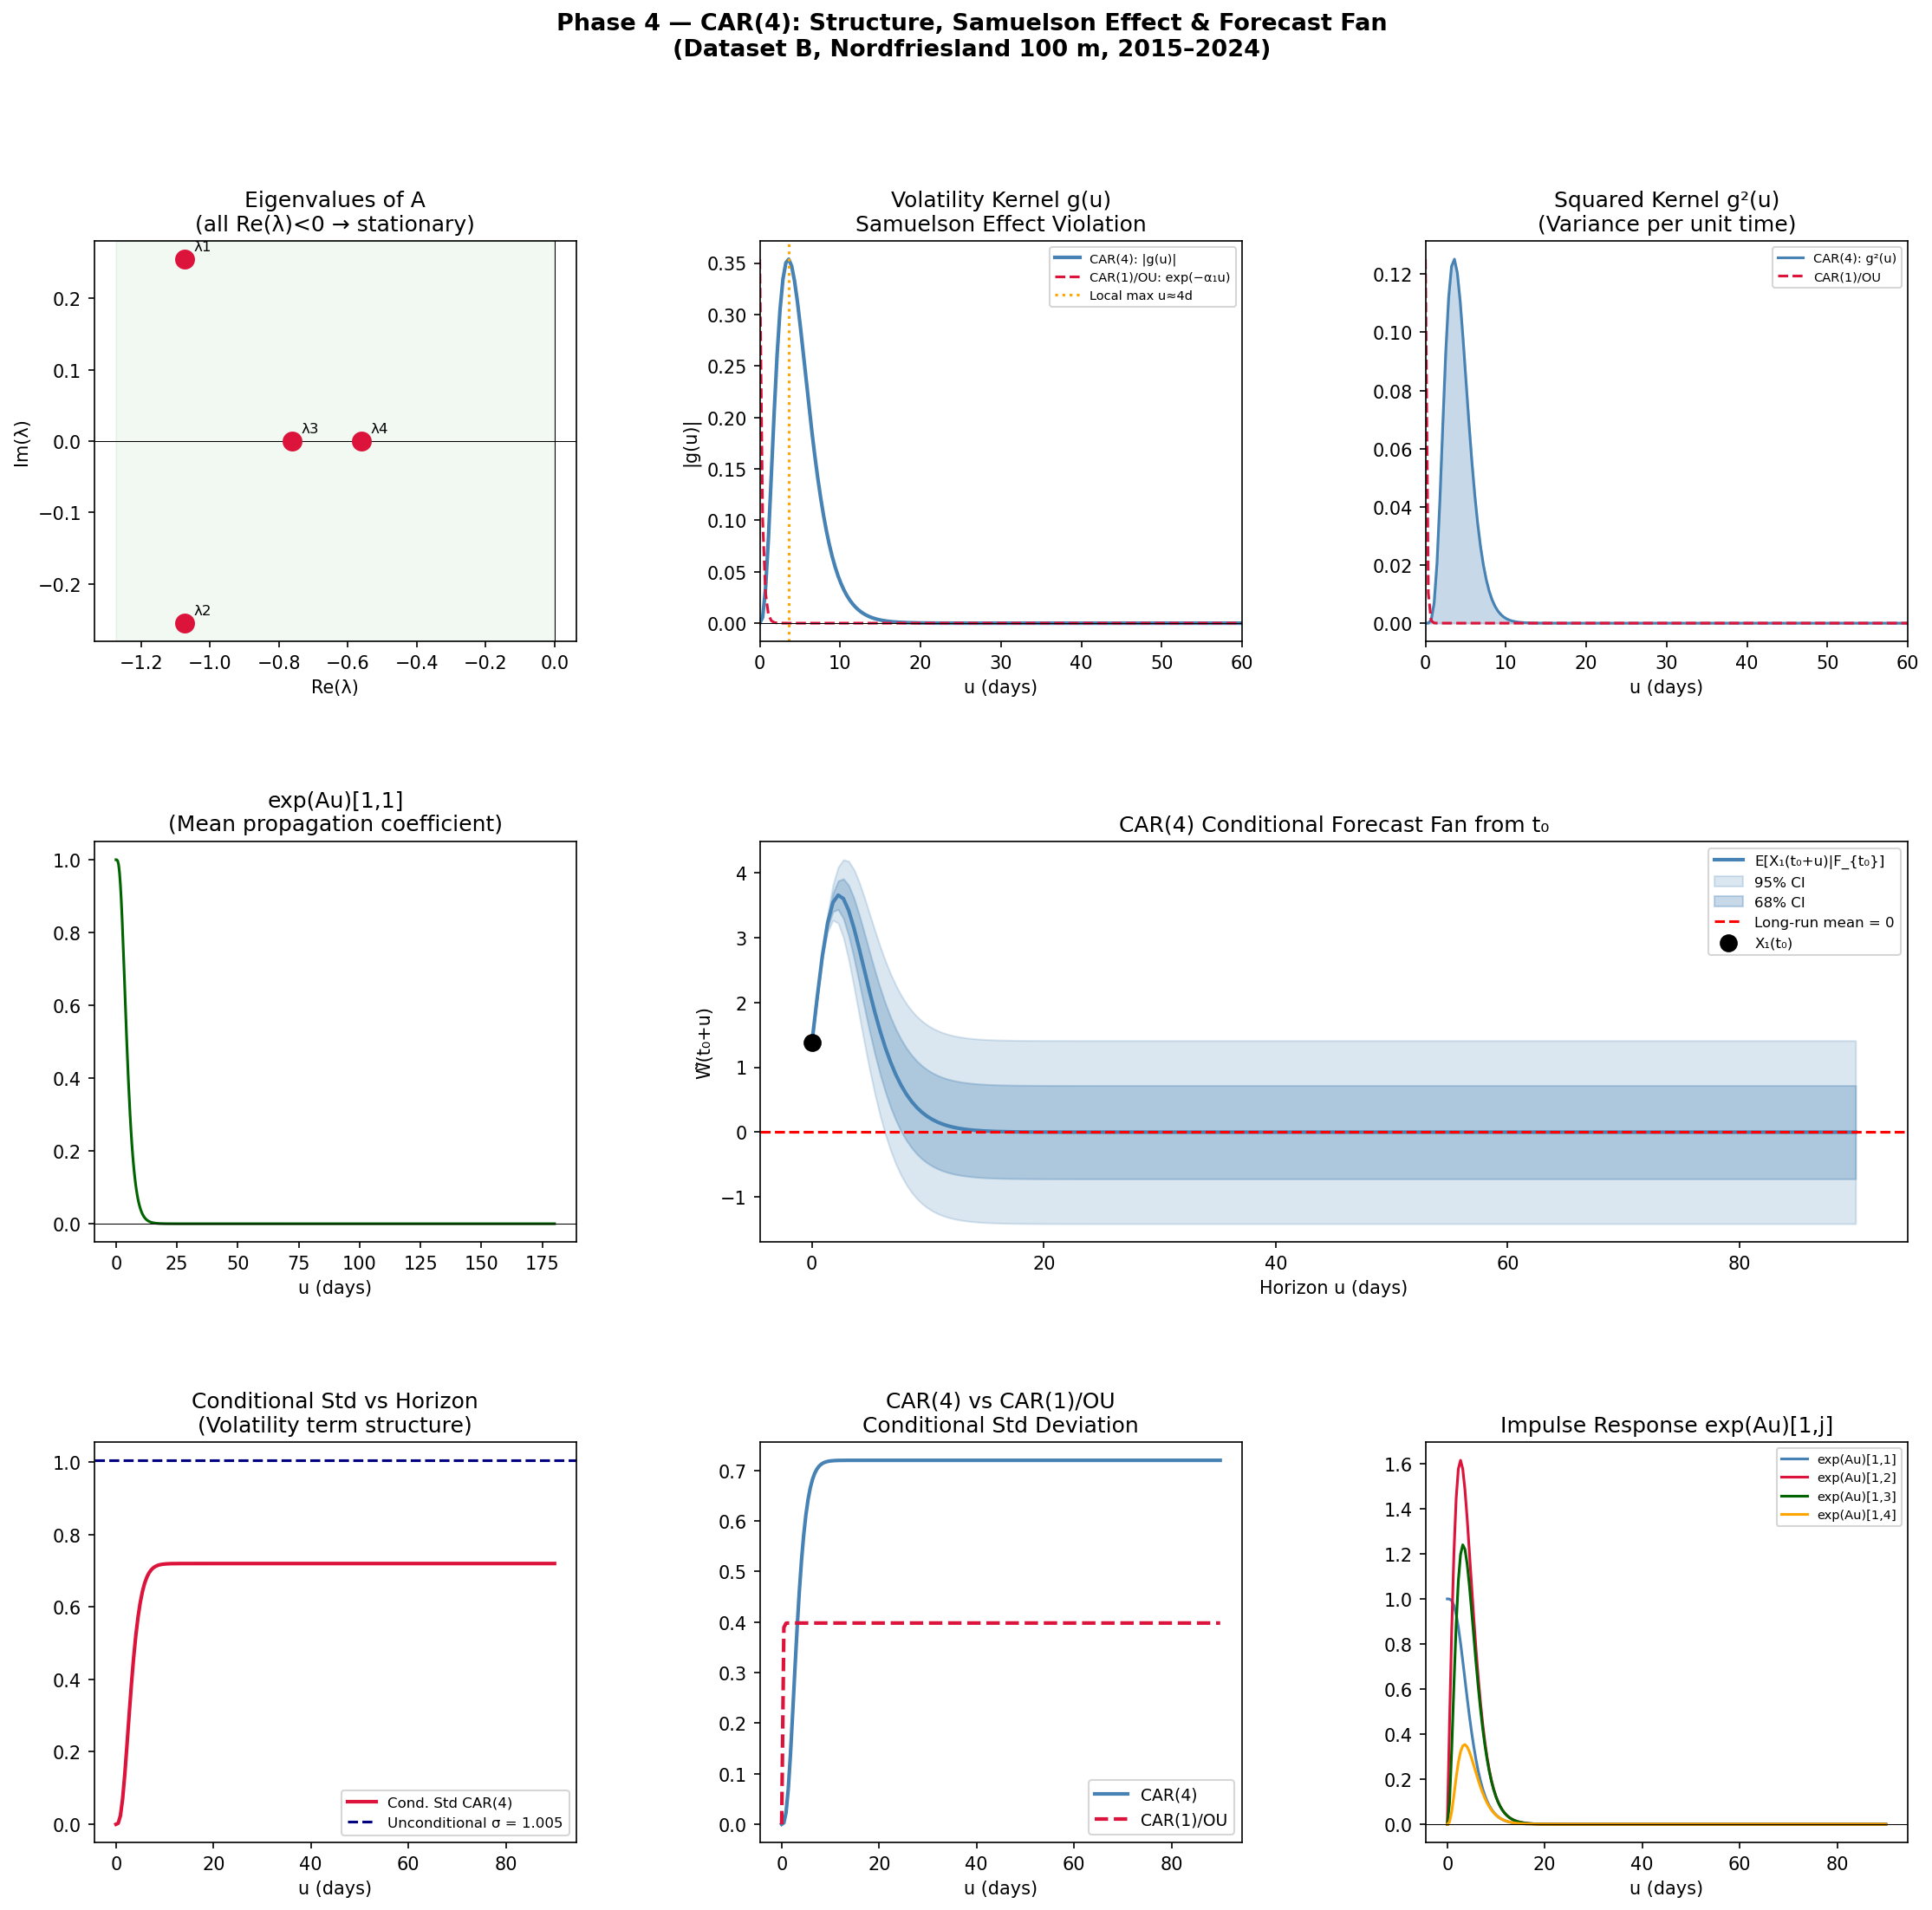
\includegraphics[width=0.95\textwidth]{../../reference_tex/Plots/phase4_B_car4_analysis.png}
\caption{\textbf{CAR(4) Stochastic Dynamics and Pricing Framework.}
\textit{Top row, left:} Eigenvalues of companion matrix $A$ in the complex plane, all with $\mathbb{Re}(\lambda) < 0$ (stationarity).
\textit{Top row, centre:} Volatility kernel $g(u) = e_1^{\top} \exp(Au) e_4$ (blue) vs.\ CAR(1)/OU baseline (red dashed), showing non-monotonic behaviour and Samuelson effect violation at $u \approx 3.6$ days.
\textit{Top row, right:} Squared kernel $g^2(u)$ governing variance accumulation.
\textit{Middle row, left:} Matrix exponential $\exp(Au)[1,1]$ showing mean propagation.
\textit{Middle row, centre--right:} Conditional forecast fan from $t_0$: mean (blue), 68\% CI (light blue), 95\% CI (lighter blue), and long-run mean at 0 (red dashed). Strong near-term predictability decays by day 14.
\textit{Bottom row:} (left) Conditional standard deviation vs.\ horizon, approaching unconditional $\sigma \approx 0.92$; (centre) CAR(4) vs.\ CAR(1) term structures; (right) impulse response matrix $\exp(Au)[1,j]$ showing oscillatory and exponential components. Dataset B, Nordfriesland 100\,m, 2015--2024.}
\label{fig:car4_analysis}
\end{figure}

\section{Conclusion}

Phase 4 translates the discrete AR(4)--GARCH system into continuous-time CAR(4) SDEs, enabling classical derivatives pricing. The Euler discretisation provides an exact, invertible mapping from AR coefficients to CAR parameters. The four eigenvalues of the companion matrix (all with negative real parts) confirm strict stationarity. Conditional forecasts exhibit strong one-day predictability, converging to the long-run mean by two weeks, consistent with synoptic weather timescales.

The non-monotonic volatility kernel $g(u)$, a hallmark of CAR($p \geq 2$), violates the classical Samuelson effect and has direct implications for the term structure of wind derivative prices. The NIG distribution, while near-Gaussian for Dataset B, provides the moment-generating function infrastructure required for the Carr--Lee (2009) characteristic-function framework in Phase 6.

The three key outputs---CAR(4) parameters, companion matrix $A$, and conditional forecast table---seed Phases 5 (theoretical stochastic volatility system) and Phase 6 (variance swap pricing), completing the model architecture.

\section*{References}

\begin{thebibliography}{99}

\bibitem{BarnNielsen:2001}
Barndorff--Nielsen, O. E., \& Shephard, N. (2001). Non-Gaussian Ornstein--Uhlenbeck-based models and some of their uses in financial economics. \textit{Journal of the Royal Statistical Society: Series B (Statistical Methodology)}, 63(2), 167--241.

\bibitem{Benth:2009}
Benth, F. E., \& Šaltytė Benth, J. (2009). Dynamic pricing of wind futures. \textit{Energy Economics}, 31(1), 16--24.

\bibitem{Brockwell:2005}
Brockwell, P. J., \& Marquardt, T. (2005). Lévy-driven and fractionally integrated ARMA processes with continuous time parameter. \textit{Statistica Sinica}, 15(3), 477--494.

\bibitem{CarrLee:2009}
Carr, P., \& Lee, R. (2009). Volatility derivatives. \textit{Annual Review of Financial Economics}, 1, 319--339.

\bibitem{Tol:1997}
Tol, R. S. J. (1997). On the autoregressive modelling of stochastic hourly wind speed series. \textit{Journal of Wind Engineering and Industrial Aerodynamics}, 68(1), 1--13.

\bibitem{SaltyteBenth:2008}
Šaltytė Benth, J., \& Benth, F. E. (2008). Stochastic modelling of temperature variations with a view towards weather derivatives. \textit{Applied Mathematical Finance}, 15(5-6), 505--525.

\end{thebibliography}

\end{document}
